\section{Definition of the signal regions}
\label{sec:sigregion}

We define signal regions to look for possible
new physics contributions by adding the requirement of large MET to the preselection. 

We define two signal regions for our search:
\begin{itemize}
\item MET $>$ 100 GeV (loose signal region):

In this region there is a small contribution from the tail of the MET distribution 
in \Z plus jets events. 
The bulk of the events in this region are from \ttbar\ events where the leptons happen to be in the \Z 
mass window.

The dilepton mass distributions for data and MC events in the loose signal region are displayed in Fig.~\ref{fig:dilmass100}.

\item MET $>$ 200 GeV (tight signal region):
This signal region was selected by picking a region where the SM expectation is very low.
At this kinematical region the dominant background contribution is expected to be from \ttbar.

\end{itemize}

In the two signal regions above, the dominant background is \ttbar. 
However, it is still essential to have a data driven estimation of the \Z contribution
in the signal regions, since if we were to observe an excess we would need to demonstrate
that this excess is not due to SM $Z$ production accompanied by artificial MET.

\begin{figure}[hbt]
\begin{center}
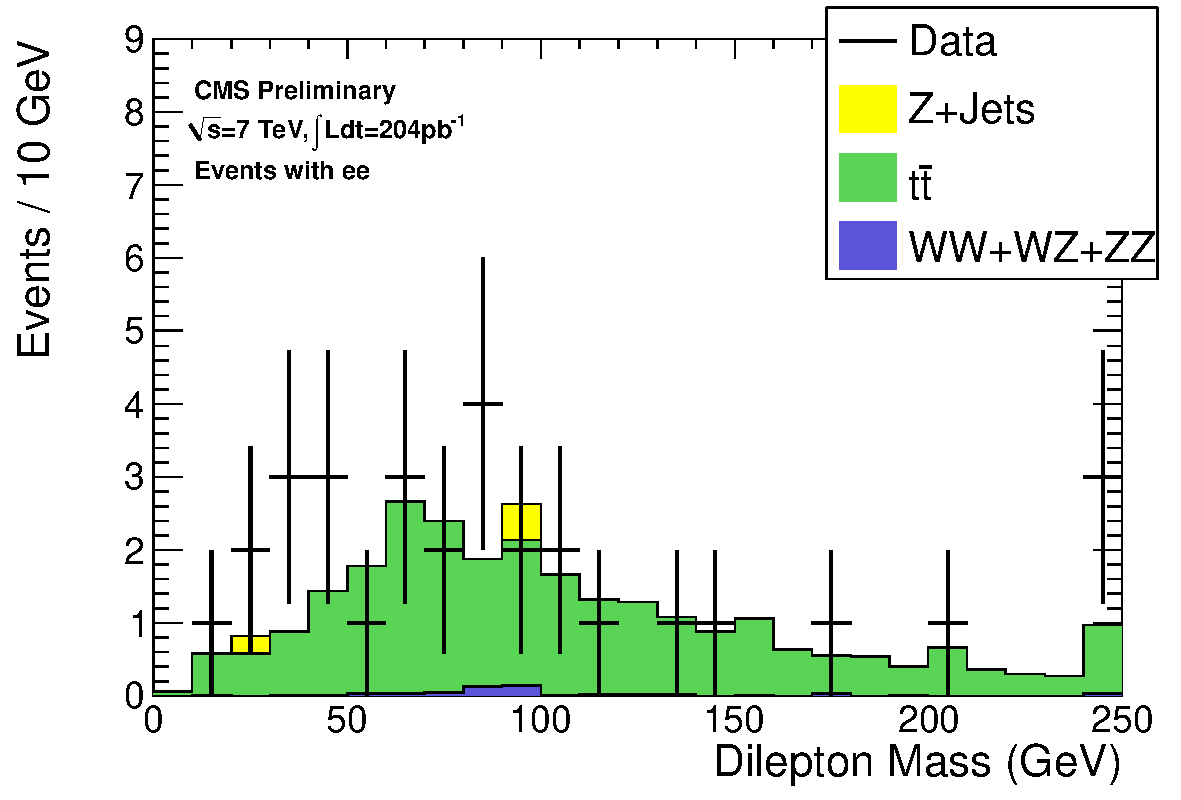
\includegraphics[width=0.48\linewidth]{plots/hdilmass_pfmet100_ee_allj.pdf}
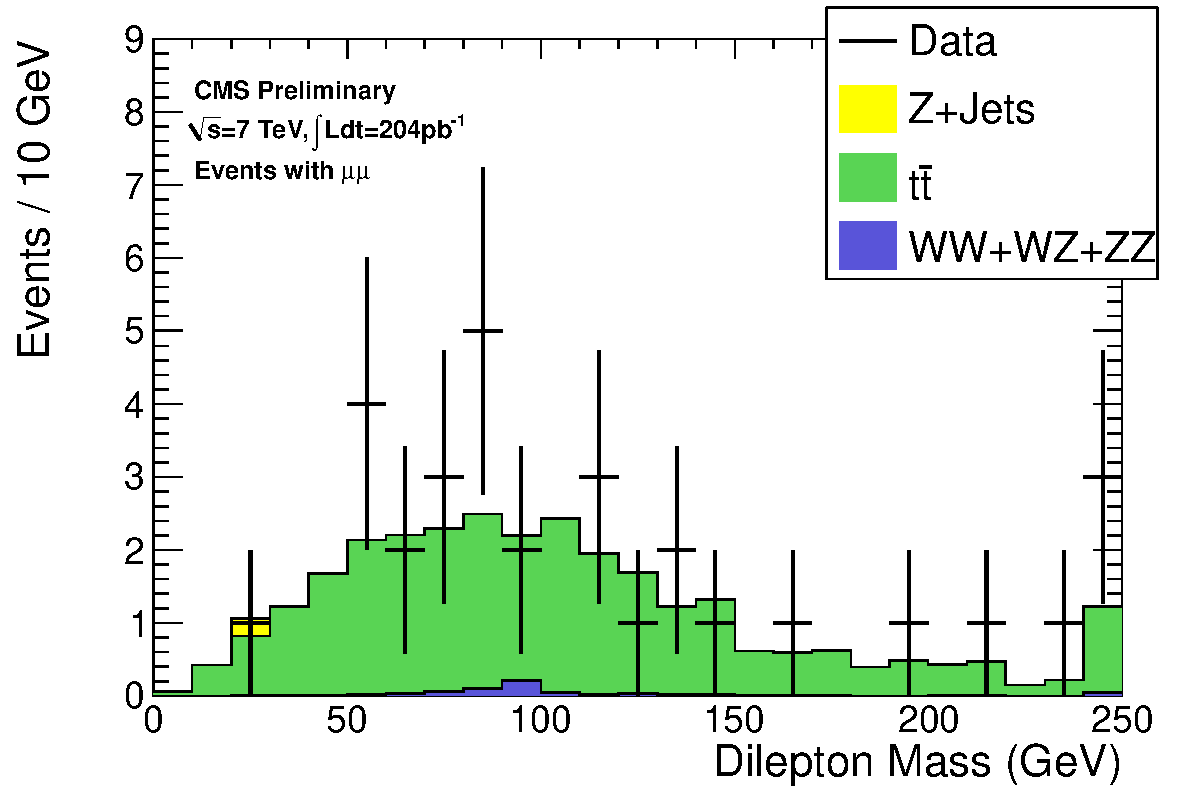
\includegraphics[width=0.48\linewidth]{plots/hdilmass_pfmet100_mm_allj.pdf}
\caption{\label{fig:dilmass100}\protect Dilepton mass distribution for events passing the pre-selection 
  and MET $>$ 100~GeV in the $ee$ (left) and $\mu\mu$ (right) final states. 
Backgrounds from single top and $W$+jets are omitted since they are negligible.}
\end{center}
\end{figure}
